%%%%% slides template
% Giovanni Ramirez (ramirez@ecfm.usac.edu.gt)
% 20200828
% Require: images/ecfmByN.png images/usacByN.jpg
%
%
% Use this option to print notes only
% \documentclass[xcolor=dvipsnames,handout,notes=only]{beamer}%
%
% Use this option to print notes and slides
% \documentclass[xcolor=dvipsnames,handout,notes=show]{beamer}%
%
% Use this option to get a printer-friendly version
% \documentclass[xcolor=dvipsnames,handout]{beamer}%
%
% Unse this option to get slides only
\documentclass[xcolor=dvipsnames,presentation]{beamer}%
%
%%%%%


%%%%% theme and coloring
% a list of themes can be found here https://hartwork.org/beamer-theme-matrix/
% I like a simple Malmoe with some modifications and color-schemes like
% dolphin for a white background, beetle for a gray background or dove for
% plain slides
%
% theme definition
\usetheme{Malmoe}
%
% definition of the presentation mode: full slides
\mode<presentation> {
% coloring for slides other options: beetle, dove
  \usecolortheme{dolphin}
% to include a slide with the table of contents
 \AtBeginSection[] {
  \begin{frame}
    \tableofcontents[currentsection]
  \end{frame} }
}
%
% definition of the handout mode: printer-friendly
\mode<handout>{
% coloring: dove is white
  \usecolortheme{dove}
% this is to print 2 slides in 1 page, other values are allowed
  \usepackage{pgfpages}
  \renewcommand\textbullet{\ensuremath{\bullet}}
  \pgfpagesuselayout{2 on 1}[letterpaper,border shrink=5mm]
% set the fontsize of the notes
  \setbeamerfont{note page}{size=\scriptsize}
% disable the slide with the table of contents
  \AtBeginSection[]{}
}
%%%%%

%%%%% personalisation
% clear all headers
\setbeamertemplate{headline}{}
% disable navigation buttons
\setbeamertemplate{navigation symbols}{}
% configure the blocks used for equations, theorems, etc
\setbeamertemplate{blocks}[rounded][shadow=true]
% clear the footline
\setbeamertemplate{footline}{}
% set the footline
\setbeamertemplate{footline}{
  \hbox{%
% left block with the shortname, it is set in the \author command
    \begin{beamercolorbox}[wd=.40\paperwidth,ht=2.25ex,dp=1ex,center]%
      {author in head/foot}%
      \usebeamerfont{author in head/foot}\insertshortauthor
    \end{beamercolorbox}%
% center block with the short title, it is set in the \title command
    \begin{beamercolorbox}[wd=.50\paperwidth,ht=2.25ex,dp=1ex,center]%
      {title in head/foot}%
      \usebeamerfont{title in head/foot}\insertshorttitle
    \end{beamercolorbox}%
% right block with the number of slides
    \begin{beamercolorbox}[wd=.10\paperwidth,ht=2.25ex,dp=1ex,right]%
      {date in head/foot}%
      \usebeamerfont{date in head/foot}
      \insertframenumber{} / \inserttotalframenumber\hspace*{1em}
    \end{beamercolorbox}}%
  \vskip0pt%
}
%%%%%

%%%%% packages
%
% language, decimal point mark
\usepackage[spanish,es-nodecimaldot]{babel}%
%
% to use only T1 scalable fonts
\usepackage[T1]{fontenc}%
\let\Tiny=\tiny% this is a proper configuration of the tiny font size
%
% to use UTF coding, other options latin1
\usepackage[utf8]{inputenc}%
%
\usepackage{array}
% special math symbols
\usepackage{latexsym,amsfonts,amsmath}%
%
% to include graphics
\usepackage{graphicx}%
% path to images
\graphicspath{ {../images/} }
%
% to use tiks: nice to draw diagrams
\usepackage{tikz}%
\usetikzlibrary{arrows,shapes,positioning}
%
% to use SI units and physics notation
\usepackage[squaren]{SIunits}%
\usepackage{physics}%
\usepackage{multirow}
\usepackage{xcolor}
%
% to use hypenation
\usepackage{ragged2e}%
\let\raggedright=\RaggedRight%
%
\usepackage{dsfont}
% to configure the hyperref to set metadata in the PDF file
\hypersetup{%
%pdfpagemode=FullScreen,% to open the file in fullscreen
breaklinks={true},% to allow links in more than one line
%pdfstartview={Fit},% to set the slide to fit the screen
%pdfpagemode=FullScreen,% to set it to full screen
pdfauthor={Giovanni Ramirez Garcia (ramirez@ecfm.usac.edu.gt)},% author name
pdftitle={Quantum Optics aplied to Quantum Computing},% title of the talk
pdfsubject={Keynote for the talk at Lat0 group},% subject of the talk
pdfkeywords={quantum optics, quantum computing, quantum algorithms, quantum
  circuits}% keywords to categorise the contents
}
%%%%%

%%%%% Talk data
%
%title
\title[Canales cuánticos PCE]% this is the short title
{\bf Mapeos proyectivos en sistemas de qubits}% this is the long title
%
% author
\author[José Alfredo de León (ECFM-USAC)]% this is the short name
{\bf José Alfredo de León${}^1$, 
Carlos Pineda${}^2$,\\
David Dávalos${}^2$, 
Alejandro Fonseca${}^3$}% this is the long name
%
% affiliation
\institute{${}^1$Escuela de Ciencias Físicas y Matemáticas, U. de 
San Carlos de Guatemala\newline%
${}^2$Instituto de Física, U. Nacional Autónoma de México\newline
${}^3$Departamento de Física, U. Federal de Pernambuco}%
%
% date and information about the conference
\date{I Congreso Guatemalteco de Física\\09 de julio de 2021}
%%%%%


\begin{document}
% % % % % % % % % % % % % % % % % % % % % % % % % % % % % % % % % % % % % %
% Title and Outline
% % % % % % % % % % % % % % % % % % % % % % % % % % % % % % % % % % % % % %
\begin{frame}[plain]
  \titlepage %
  \begin{tikzpicture}[x=1mm,y=1mm,overlay,remember picture]
    \pgftransformshift{\pgfpointanchor{current page}{center}}
    \node[inner sep=0pt] (usac) at (-35,-30) %
    {
\includegraphics[height=12mm]{logos/ecfmByN}};
    \node[inner sep=0pt] (usac) at (0,-30) %
    {
\includegraphics[height=12mm]{logos/ifunam}};
    \node[inner sep=0pt] (ecfm) at (35,-30) %
    {
\includegraphics[height=12mm]{logos/u-pernambuco}};
  \end{tikzpicture}
\end{frame}

\begin{frame}{Outline}
  \tableofcontents[hidesubsections] 
\end{frame}


% % % % % % % % % % % % % % % % % % % % % % % % % % % % % % % % % % % % % %
% Introduction and Motivation
% % % % % % % % % % % % % % % % % % % % % % % % % % % % % % % % % % % % % %
\section{Sistemas cuánticos abiertos}
\label{sec:Intro}

\begin{frame}{Sistema cerrado}
	\vspace{-.1cm}
	\begin{center}
		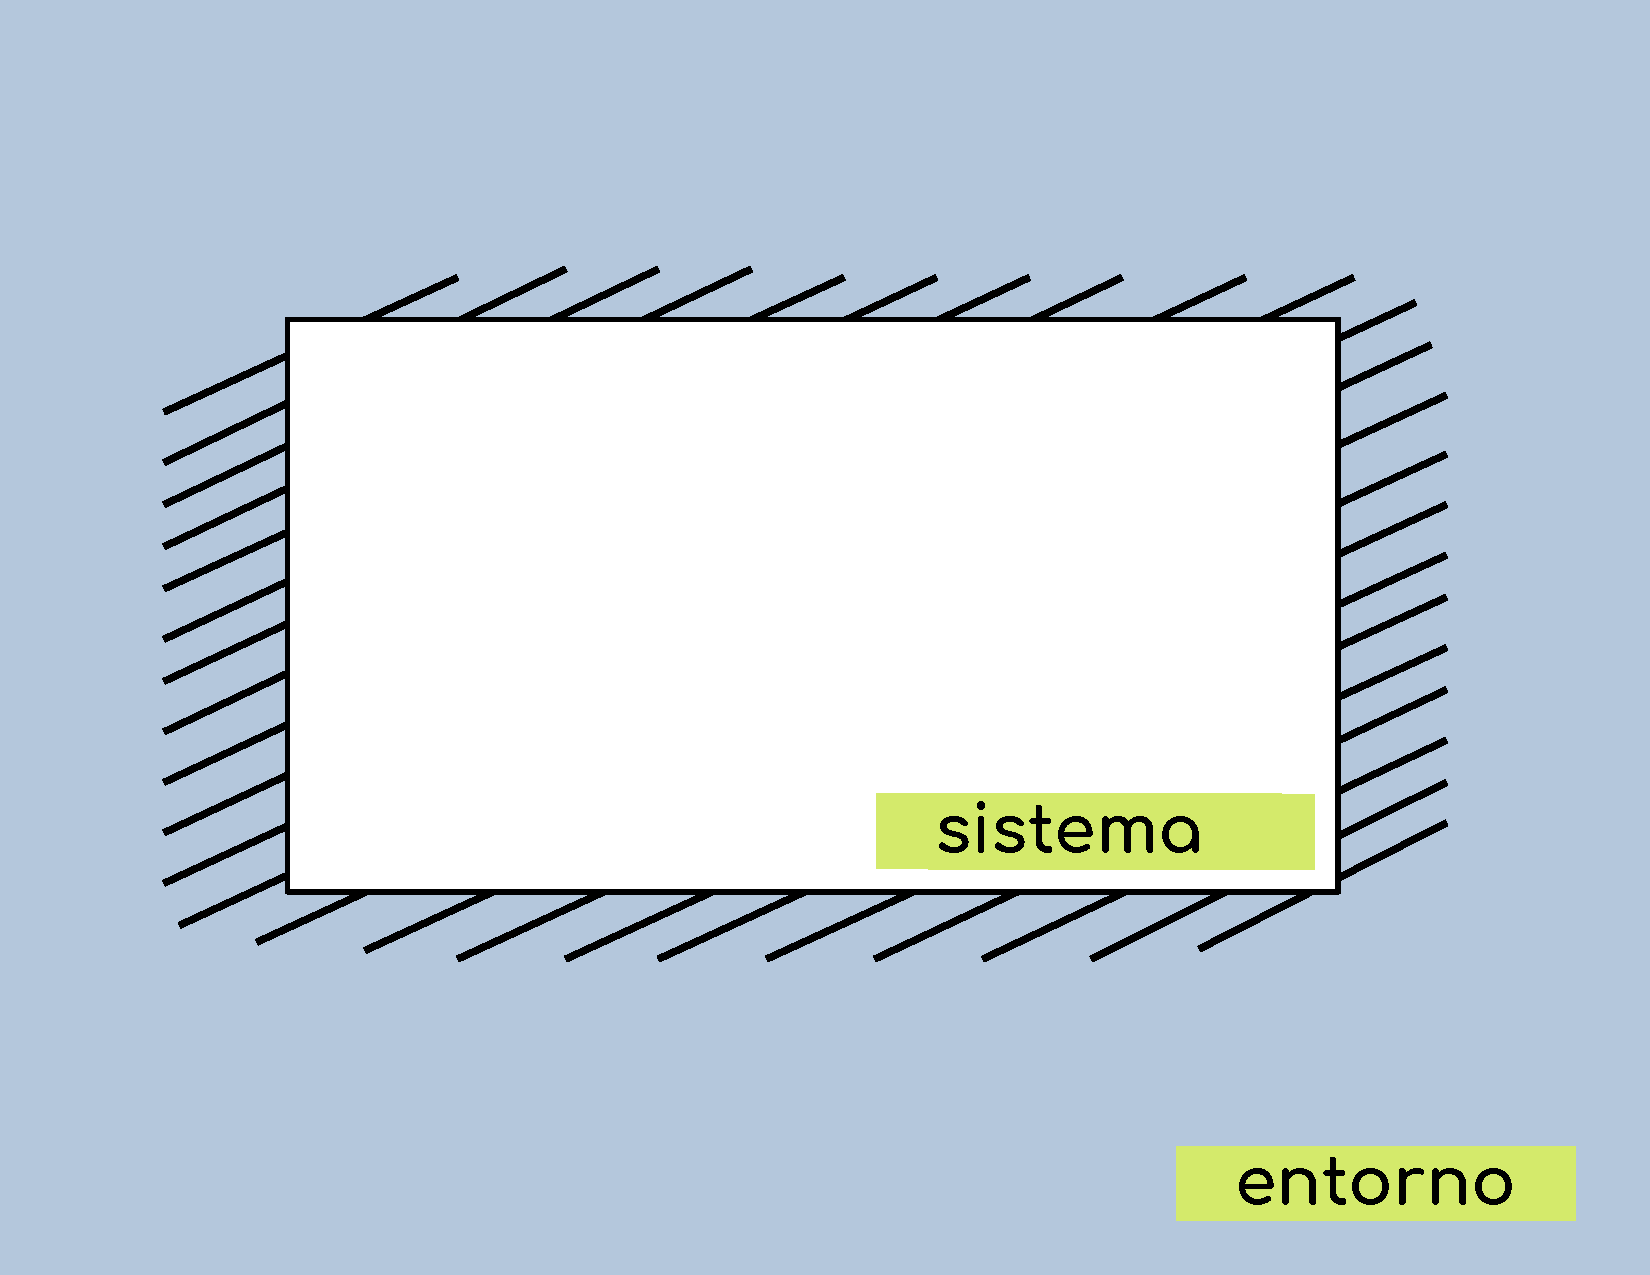
\includegraphics[height=7cm]{sistema_cerrado.pdf}
	\end{center}
\end{frame}

\begin{frame}{Sistema abierto}

	\only<1>{
	\vspace{-.1cm}
	\begin{center}
		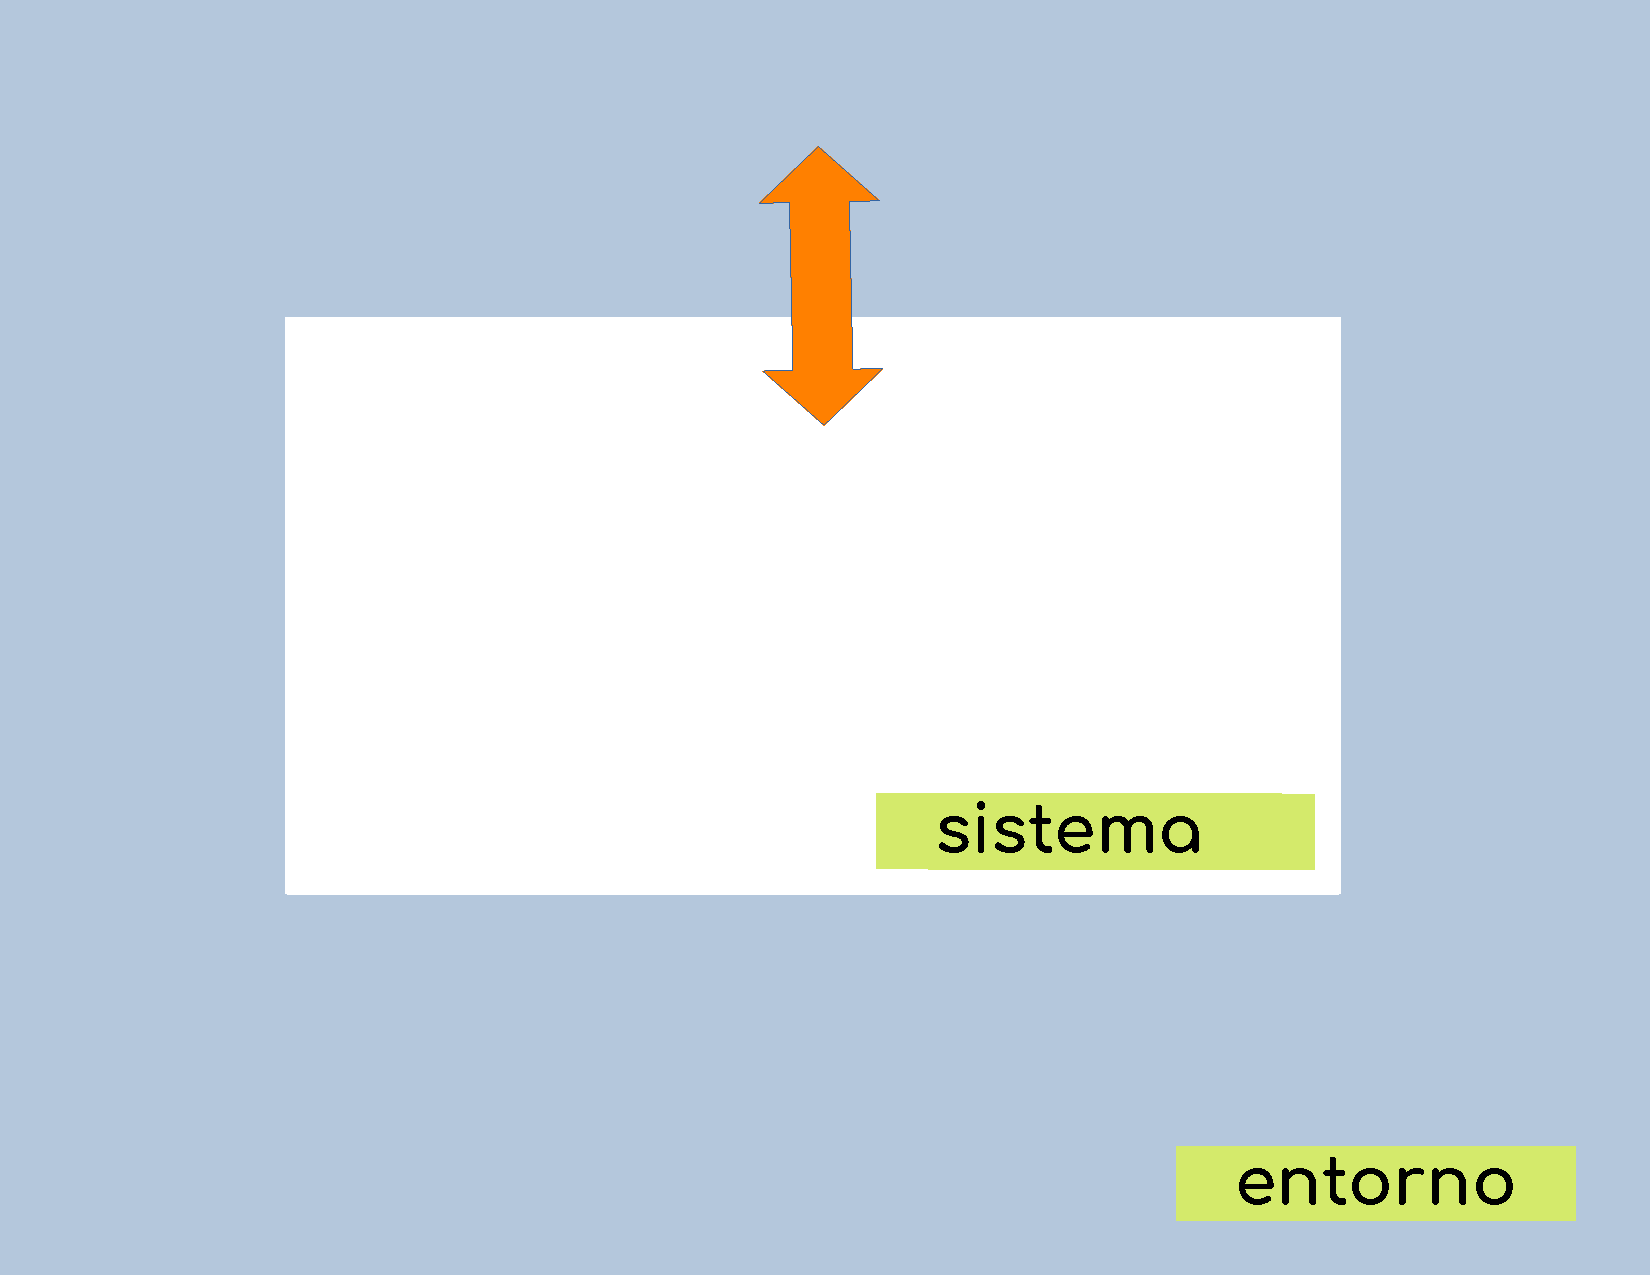
\includegraphics[height=7cm]{sistema_abierto01.pdf}
	\end{center}
  }
  
  \only<2>{
	\vspace{-.1cm}
	\begin{center}
		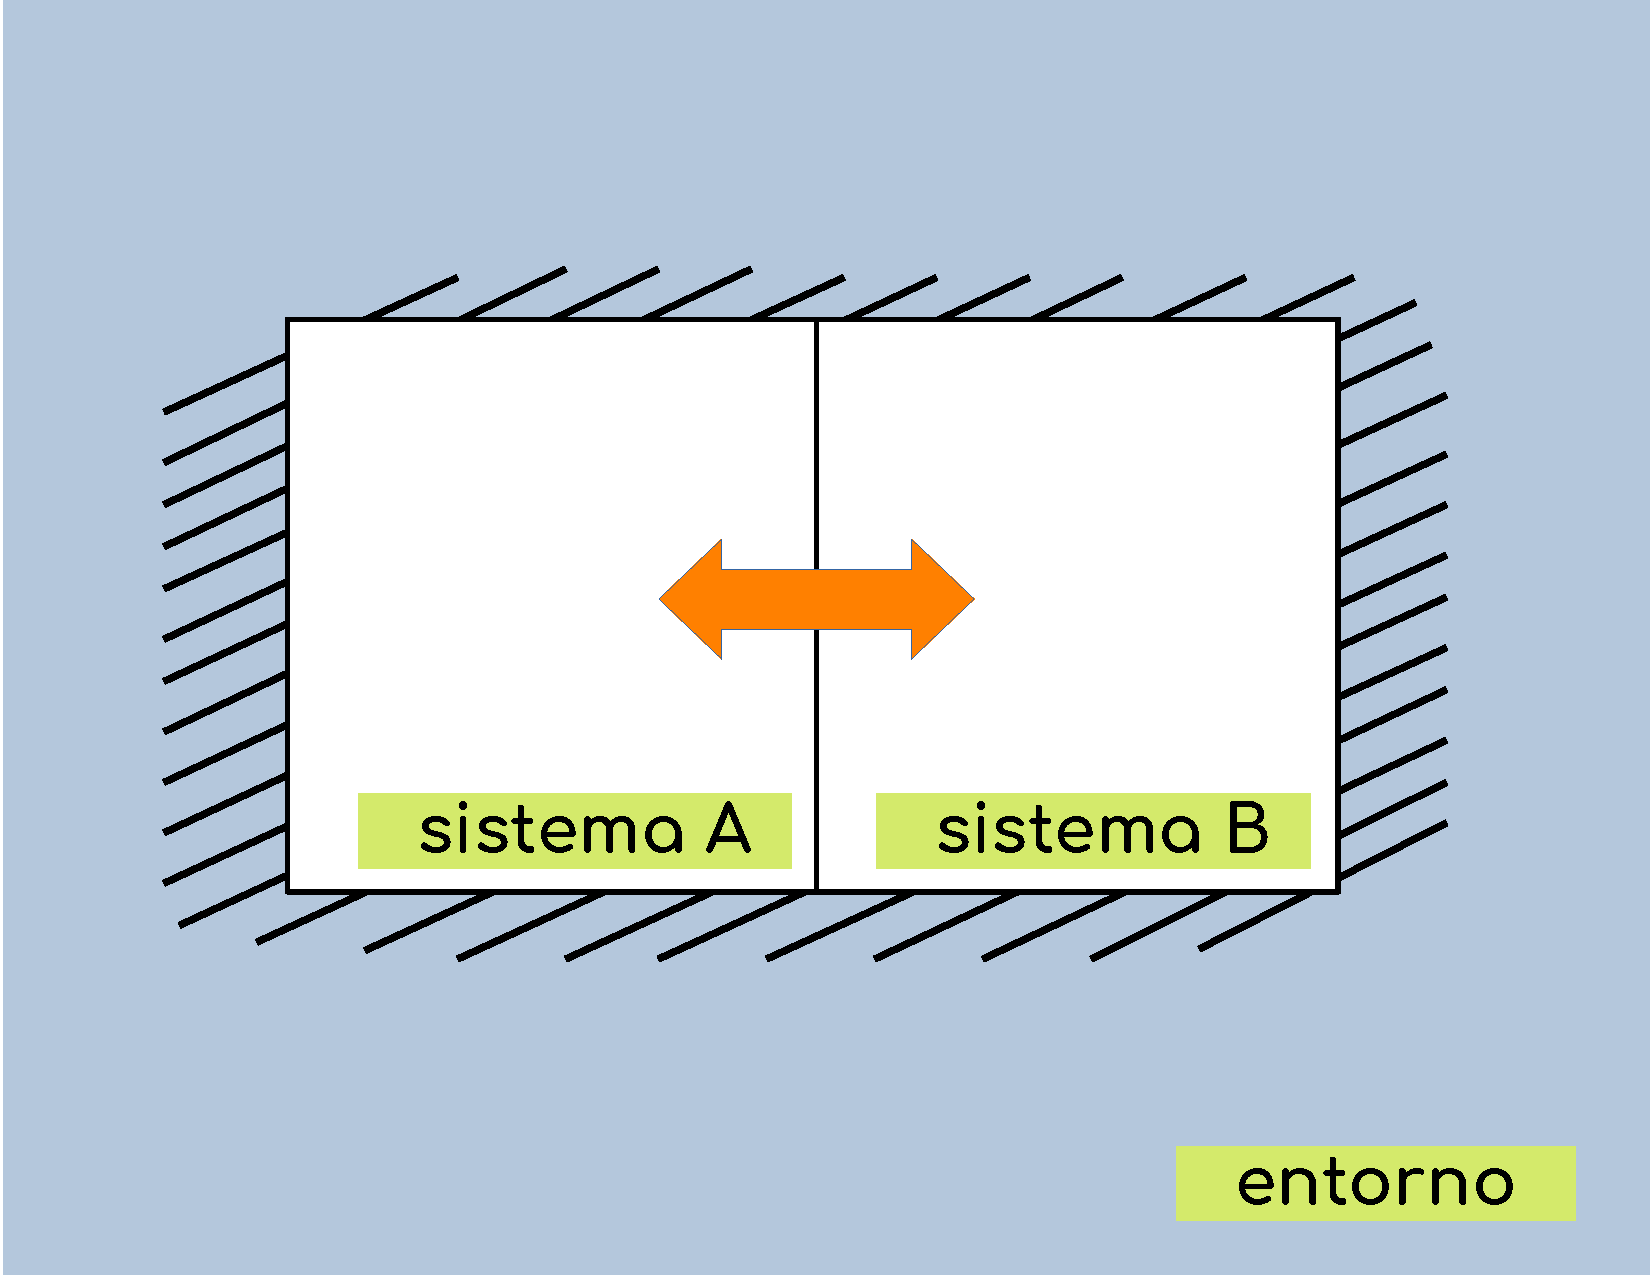
\includegraphics[height=7cm]{sistema_abierto02.pdf}
	\end{center}
  }    
  
%  \only<1>{
%  \vspace{-.6cm}
%  Sin embargo, los sistemas cuánticos reales son sistemas 
%  abiertos a interacciones con su entorno.
%  
%  \vfill
%	}
%	
%	\only<2>{
%  \vspace{-.6cm}
%  \alert{
%  Sin embargo, los sistemas cuánticos reales son sistemas 
%  abiertos a interacciones con su entorno.
%  }
%  
%  \vfill
%	}

\end{frame}


\begin{frame}{Sistemas abiertos}
{¿cómo representar a los estados?}
   \only<1>{
  La herramienta más apropiada para representar al estado de un 
  sistema cuántico abierto es la matriz de densidad $\rho$. \vfill
  
  Por ejemplo, supongamos un sistema cuyo estado es $\ket{\psi}$,
  su matriz de densidad se escribe
  \begin{align*}
  \rho=\dyad{\psi}{\psi}.
  \end{align*}
  }

	\only<2>{
	Una matriz $\rho$ representa a un estado cuántico si y sólo si 	
	\begin{enumerate}
		\item $\Tr (\rho)=1$,
		\item $\rho^{\dagger}=\rho$,
		\item $\rho\geq 0$.
	\end{enumerate}	
	}
\end{frame}


\begin{frame}{Sistemas abiertos}%
  {Dinámica}
  
  La teoría de los canales cuánticos es una forma para describir 
  la evolución de la matriz de densidad (estado cuántico). \vfill
  
  \only<1>{
	Una operación lineal $\mathcal{E}$ que actúa sobre $\rho$ 	como 
	\begin{align*}
	\mathcal{E}(\rho)=\rho'
	\end{align*}
	es un canal cuántico si
	\begin{enumerate}
	\item Preserva las características de la matriz de densidad,
	\item Es una operación completamente positiva.
	\end{enumerate}
	}
	
	\only<2>{
	Una operación lineal $\mathcal{E}$ que actúa sobre $\rho$ como 
	\begin{align*}
	\mathcal{E}(\rho)=\rho'
	\end{align*}
	es un canal cuántico si
	\begin{enumerate}
	\item \alert{Preserva las características de la matriz de densidad},
	\item Es una operación completamente positiva.
	\end{enumerate}
	}
	
	\only<3>{
	Una operación lineal $\mathcal{E}$ que actúa sobre $\rho$ 	como 
	\begin{align*}
	\mathcal{E}(\rho)=\rho'
	\end{align*}
	es un canal cuántico si
	\begin{enumerate}
	\item Preserva las características de la matriz de densidad,
	\item \alert{Es una operación completamente positiva}.
	\end{enumerate}
	}
\end{frame}	

\begin{frame}{Completa positividad}{¿Para qué o qué?}
	Supongamos una operación $\mathcal{E}$ que actúa sobre 
	el sistema A.
	
	\only<1->{
	\begin{center}
	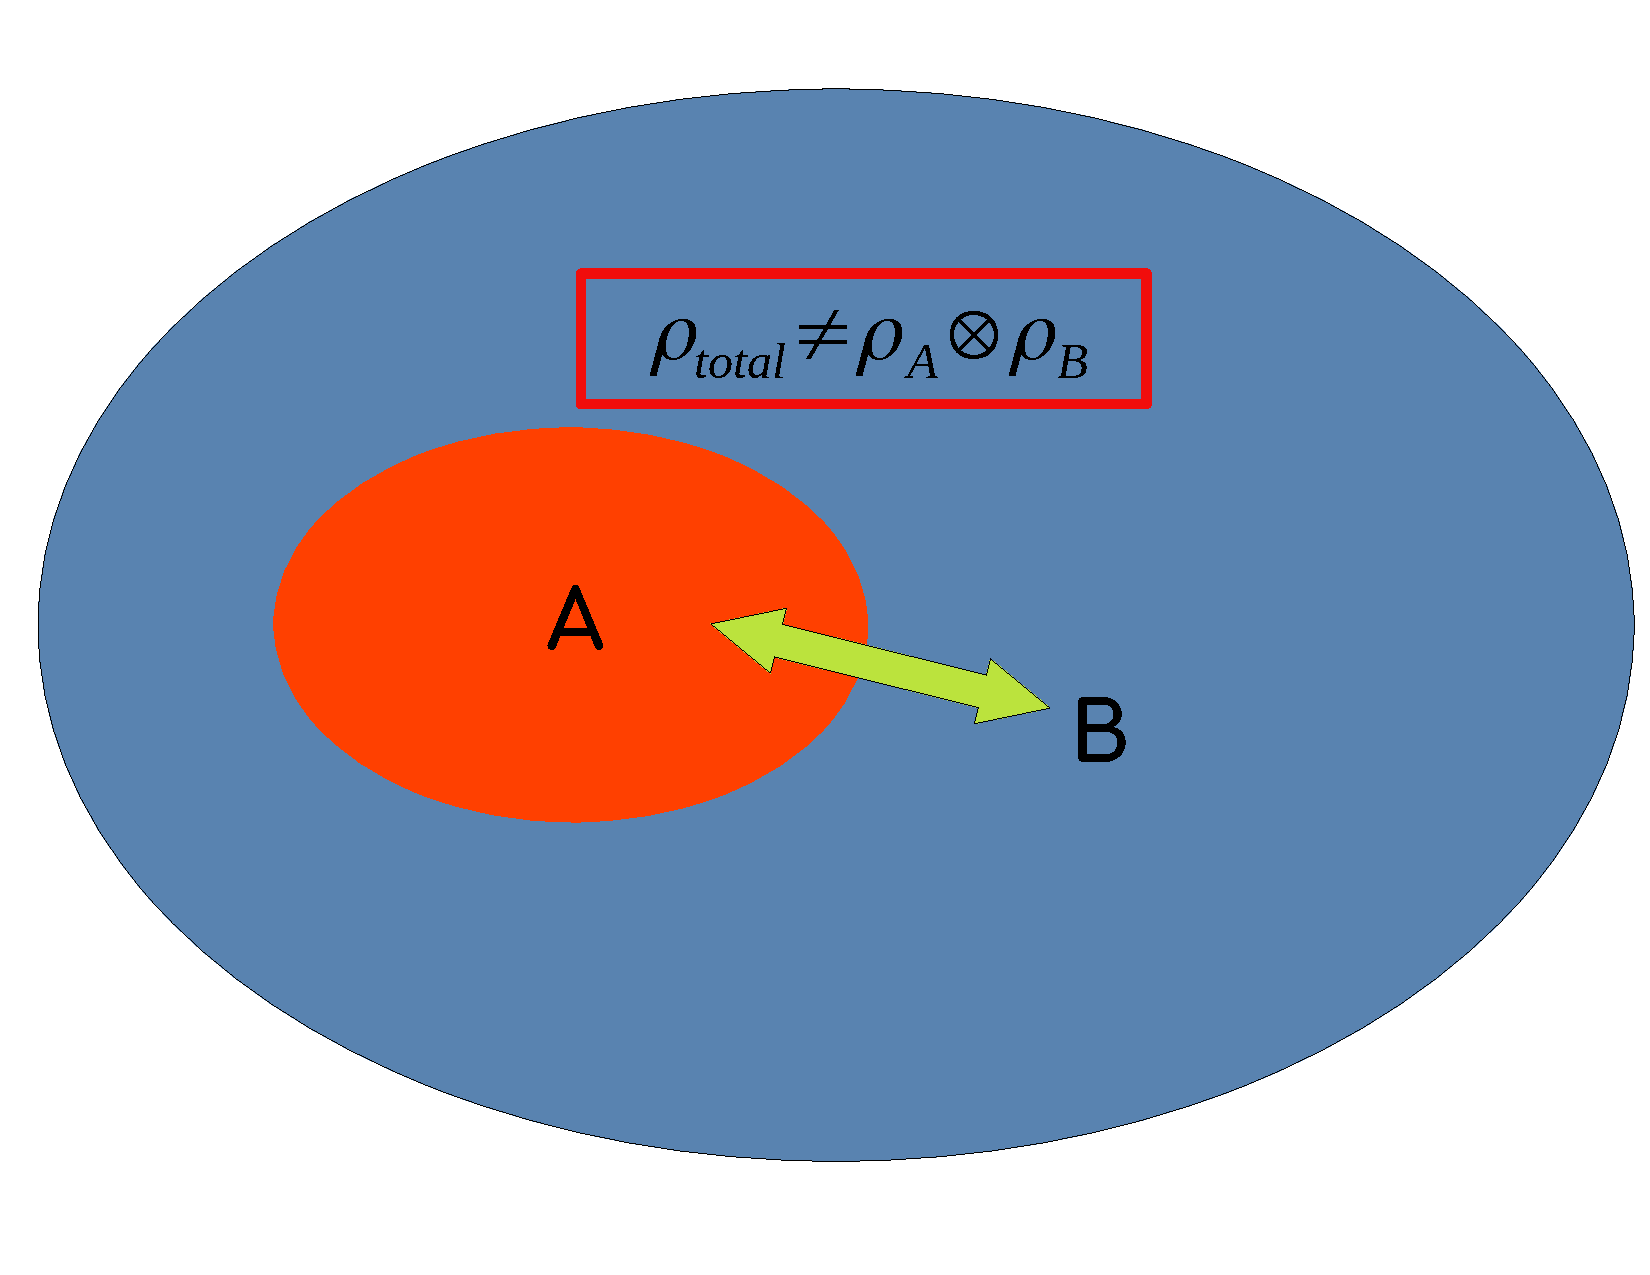
\includegraphics[height=6cm]{CP2}
	\end{center}	
	}
	
	No es suficiente que 	$\mathcal{E}(\rho_A)\geq0$, \only<1>{también 
	$\qty(\mathcal{E}\otimes \mathds{1}_k)\qty[\rho_{total}]\geq0$.}\only<2>{\alert{también 
	$\qty(\mathcal{E}\otimes \mathds{1}_k)\qty[\rho_{total}]\geq0$.}} 
\end{frame}

\begin{frame}{Canal cuántico}
	\begin{center}
		\includegraphics[width=7cm]{QuantumChannel}
	\end{center}
	\vspace{-.2cm}
	\only<1>{
	Una operación $\mathcal{E}$ es un canal cuántico si y sólo si 
	\begin{align*}
	 \qty(\mathcal{E}\otimes \mathds{1})\qty[\dyad{\text{Bell}}{\text{Bell}}]
	\hspace{.5cm}	 
	 \text{(matriz de Choi de }\mathcal{E})
	\end{align*}
	es (1) de traza unitaria, (2) Hermítica y (3) positiva.}
	\only<2>{
	Una operación $\mathcal{E}$ es un canal cuántico si y sólo si 
	\begin{align*}
	 \qty(\mathcal{E}\otimes \mathds{1})\qty[\dyad{\text{Bell}}{\text{Bell}}]
	\hspace{.5cm}	 
	 \alert{\text{(matriz de Choi de }\mathcal{E})}
	\end{align*}
	es (1) de traza unitaria, (2) Hermítica y (3) positiva.	
	}
\end{frame}


\begin{frame}{Resumen}
	\begin{enumerate}
		\item Sistemas cuánticos reales: abiertos
		\item Estados cuánticos: matriz de densidad $\rho$
		\item Dinámica: canales cuánticos
	\end{enumerate}
\end{frame}

% % % % % % % % % % % % % % % % % % % % % % % % % % % % % % % % % % % % % %
% Qubits
% % % % % % % % % % % % % % % % % % % % % % % % % % % % % % % % % % % % % %

\section{Qubits}

\begin{frame}{Qubit}
	Un qubit es un sistema cuántico de dos niveles.
	
	\begin{columns}
	\hspace{1cm}
	\begin{column}{0.7\textwidth}
		\begin{align*}
			\rho &= \frac{\mathds{1}+r_1\sigma_x+r_2\sigma_y+r_3\sigma_z}{2},
		\end{align*}	
		$\qty(r_1,r_2,r_3)$ especifican las coordenadas cartesianas de un 
 		punto en la esfera de Bloch,
 	\begin{align*}
 		\alert{\rho = \qty(1,r_1,r_2,r_3)}.
 	\end{align*}
	\end{column}\hspace{-1cm}
	\begin{column}{0.5\textwidth}  
  		\begin{center}
    		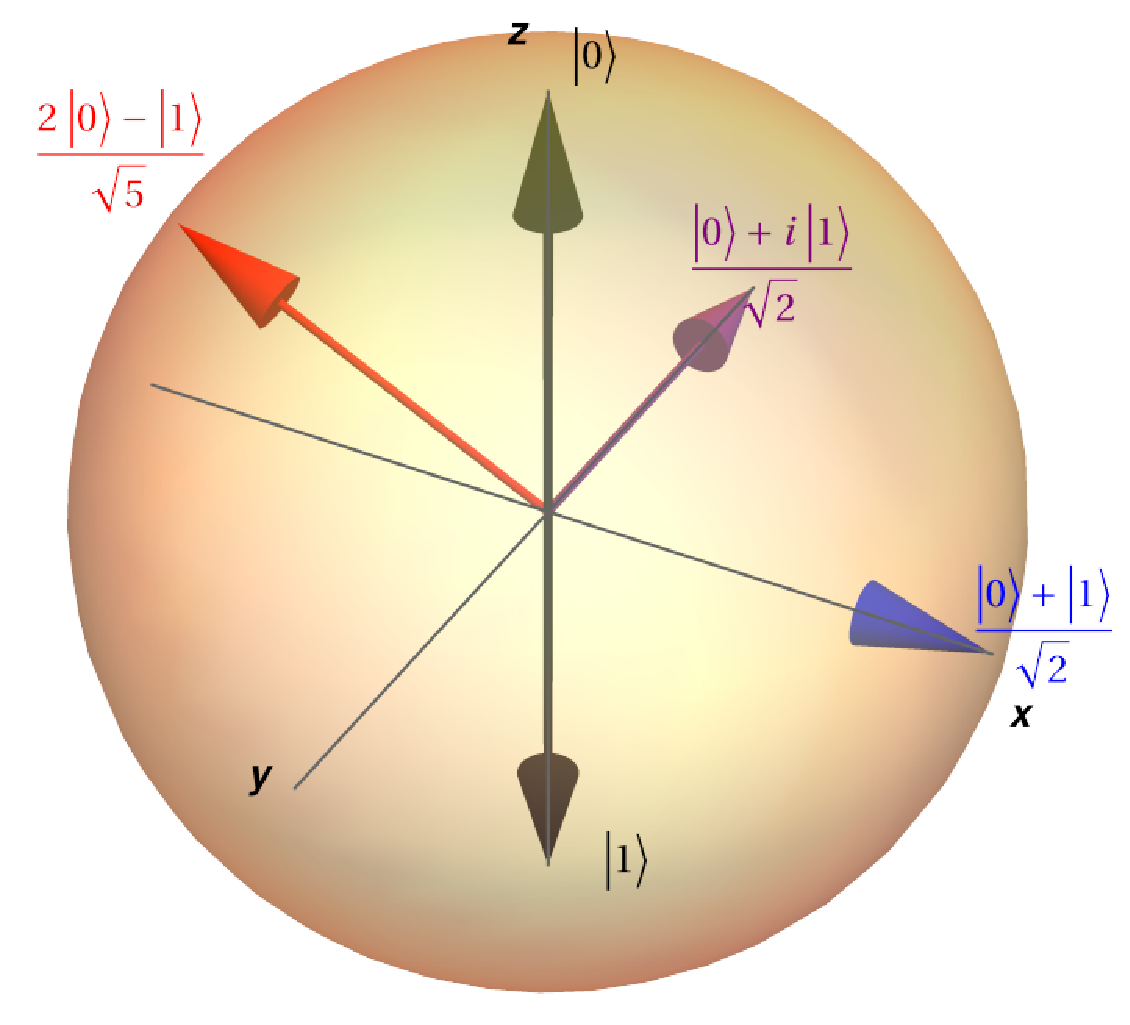
\includegraphics[width=0.7\textwidth]{bloch-sph}      
     \end{center}
		\end{column}
	\end{columns}
\end{frame}

\begin{frame}{Canal \textit{bit-flip} de 1 qubit}
	El \textit{bit-flip} actúa sobre la esfera de Bloch como
	\begin{center}
	\begin{tabular}{m{2.5cm} m{1.5cm} m{2.5cm}}
		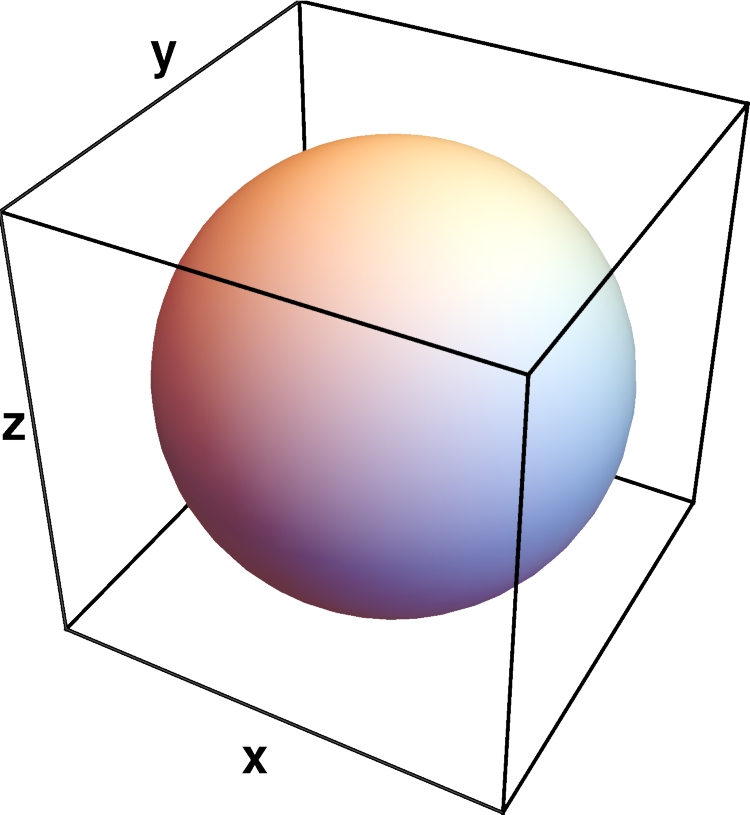
\includegraphics[width=3cm]{unit_sph}
		& \hfill \LARGE{$\longmapsto$} \hfill
		& 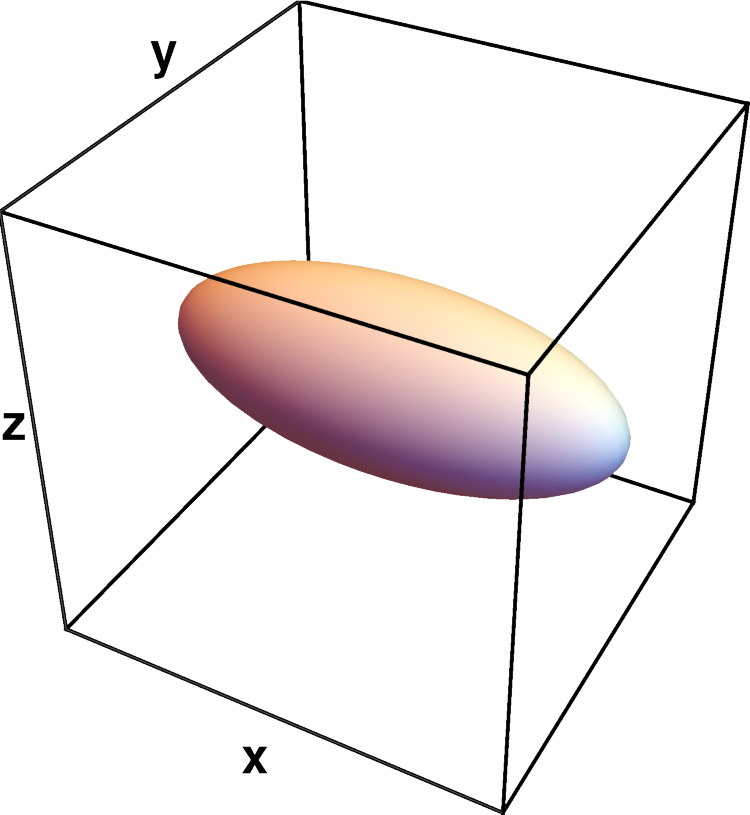
\includegraphics[width=3cm]{bit_flip_p0_3}
	\end{tabular}
	\end{center}
	
	Transforma a las componentes $r_i$ de la matriz de densidad como
	\begin{align*}
	\qty(1,r_1,r_2,r_3) \longmapsto \qty(1,r_1,\qty(1-2p)r_2,\qty(1-2p)r_3).
	\end{align*}
\end{frame}

\begin{frame}{Matriz de densidad de $n$ qubits}
	En la base de productos tensoriales de las matrices de Pauli, 
	la matriz de densidad de $n$ qubits se escribe
	\begin{align*}
		\rho = \frac{1}{2^n}\sum _{j_1,\ldots,j_n=0}^3 r_{j_1,\ldots,j_n}
		\sigma_{j_1}\otimes \ldots
		\otimes\sigma_{j_n},\hspace{.8cm} r_{0,\ldots,0}=1.
	\end{align*}
	\only<1>{Llamaremos `componentes de Pauli' a las 
	$r_{j_1,\ldots,j_n}$.}\only<2>{\alert{Llamaremos 
	`componentes de Pauli' a las $r_{j_1,\ldots,j_n}$.}}
\end{frame}

% % % % % % % % % % % % % % % % % % % % % % % % % % % % % % %
% Operaciones PCE
% % % % % % % % % % % % % % % % % % % % % % % % % % % % % % % 
\section{Operaciones PCE}
\label{sec:Theory}

\begin{frame}{Motivación (1/2)}
	Un caso particular del canal \textit{bit-flip} es cuando
	\begin{center}
	\begin{tabular}{m{2.5cm} m{1.5cm} m{2.5cm}}
		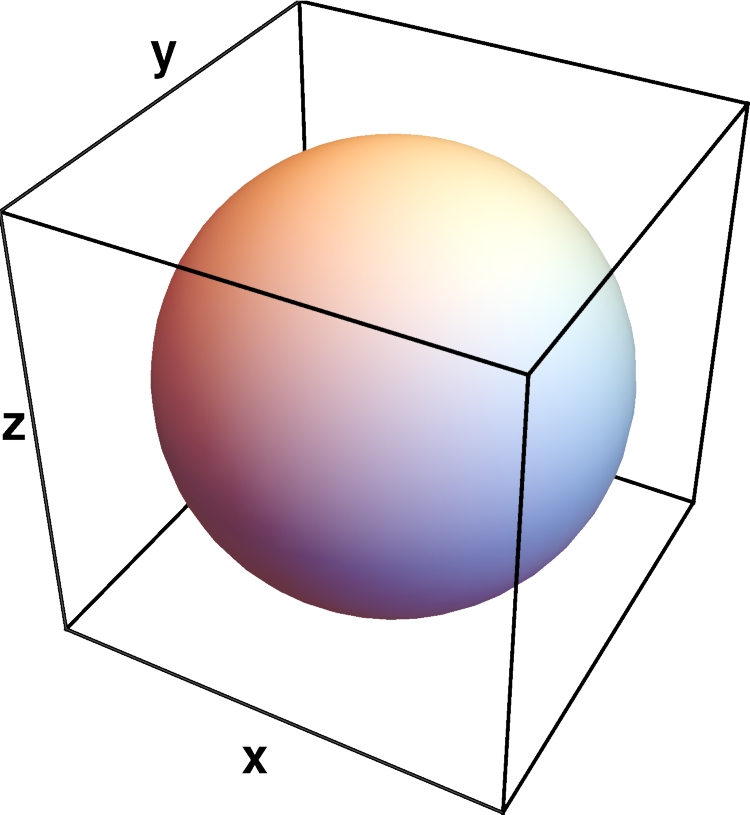
\includegraphics[width=3cm]{unit_sph}
		& \hfill \LARGE{$\longmapsto$}
		& 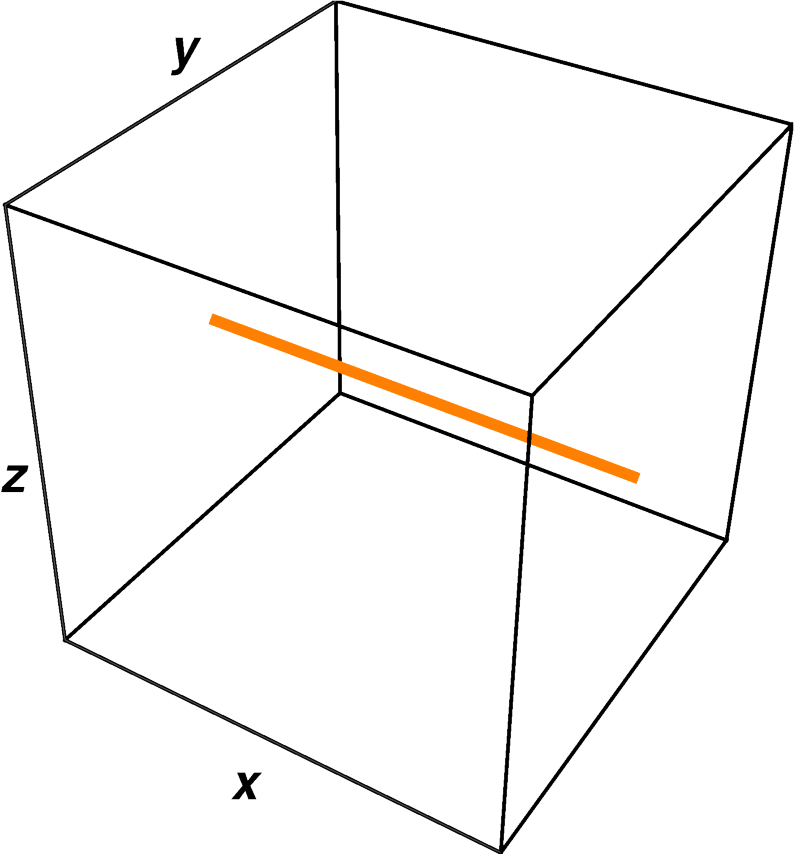
\includegraphics[width=3cm]{bit_flip_p0_5}
	\end{tabular}
	\end{center}
	
	Las componentes de Pauli $r_i$ se transforman como
	\begin{align*}
	\qty(1,r_1,r_2,r_3)\longmapsto \qty(1,r_1,0,0).
	\end{align*}
	
	\onslide<2>{
	\alert{¿Son canales cuánticos todas las operaciones que borran
	cualesquiera de las componentes de Pauli de 1 qubit?}
	}

\end{frame}


\begin{frame}{Motivación (2/2)}
	\only<1>{\alert{No.}}\only<2>{No.}
	Las operaciones $\Lambda$ que borran dos componentes de Pauli no 
	son canales cuánticos.
	\begin{center}
	\begin{tabular}{m{2.5cm} m{1.3cm} m{2.5cm}}
		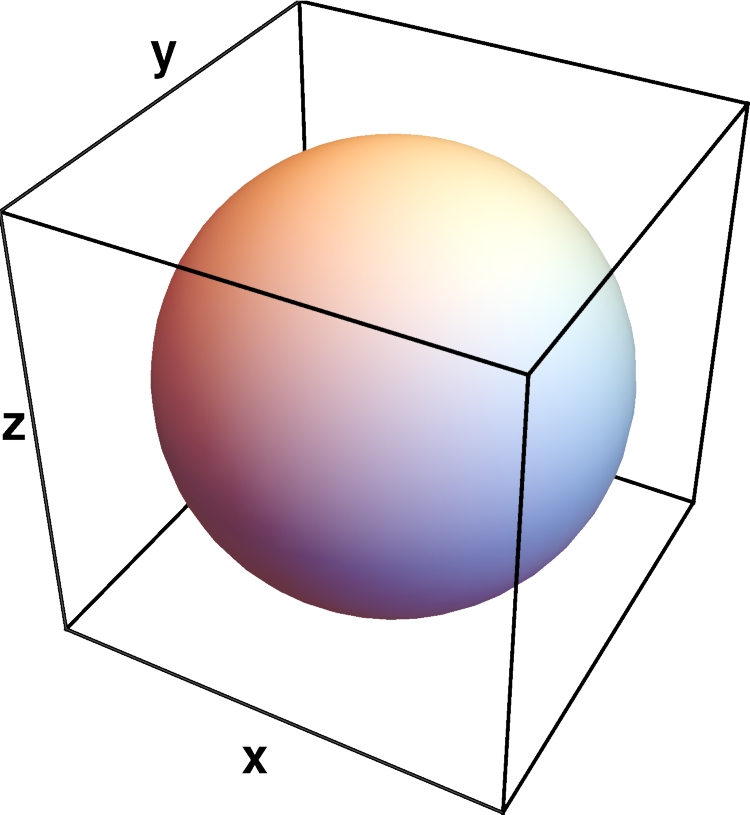
\includegraphics[width=3cm]{unit_sph}
		& \hfill \LARGE{$\longmapsto$}
		& 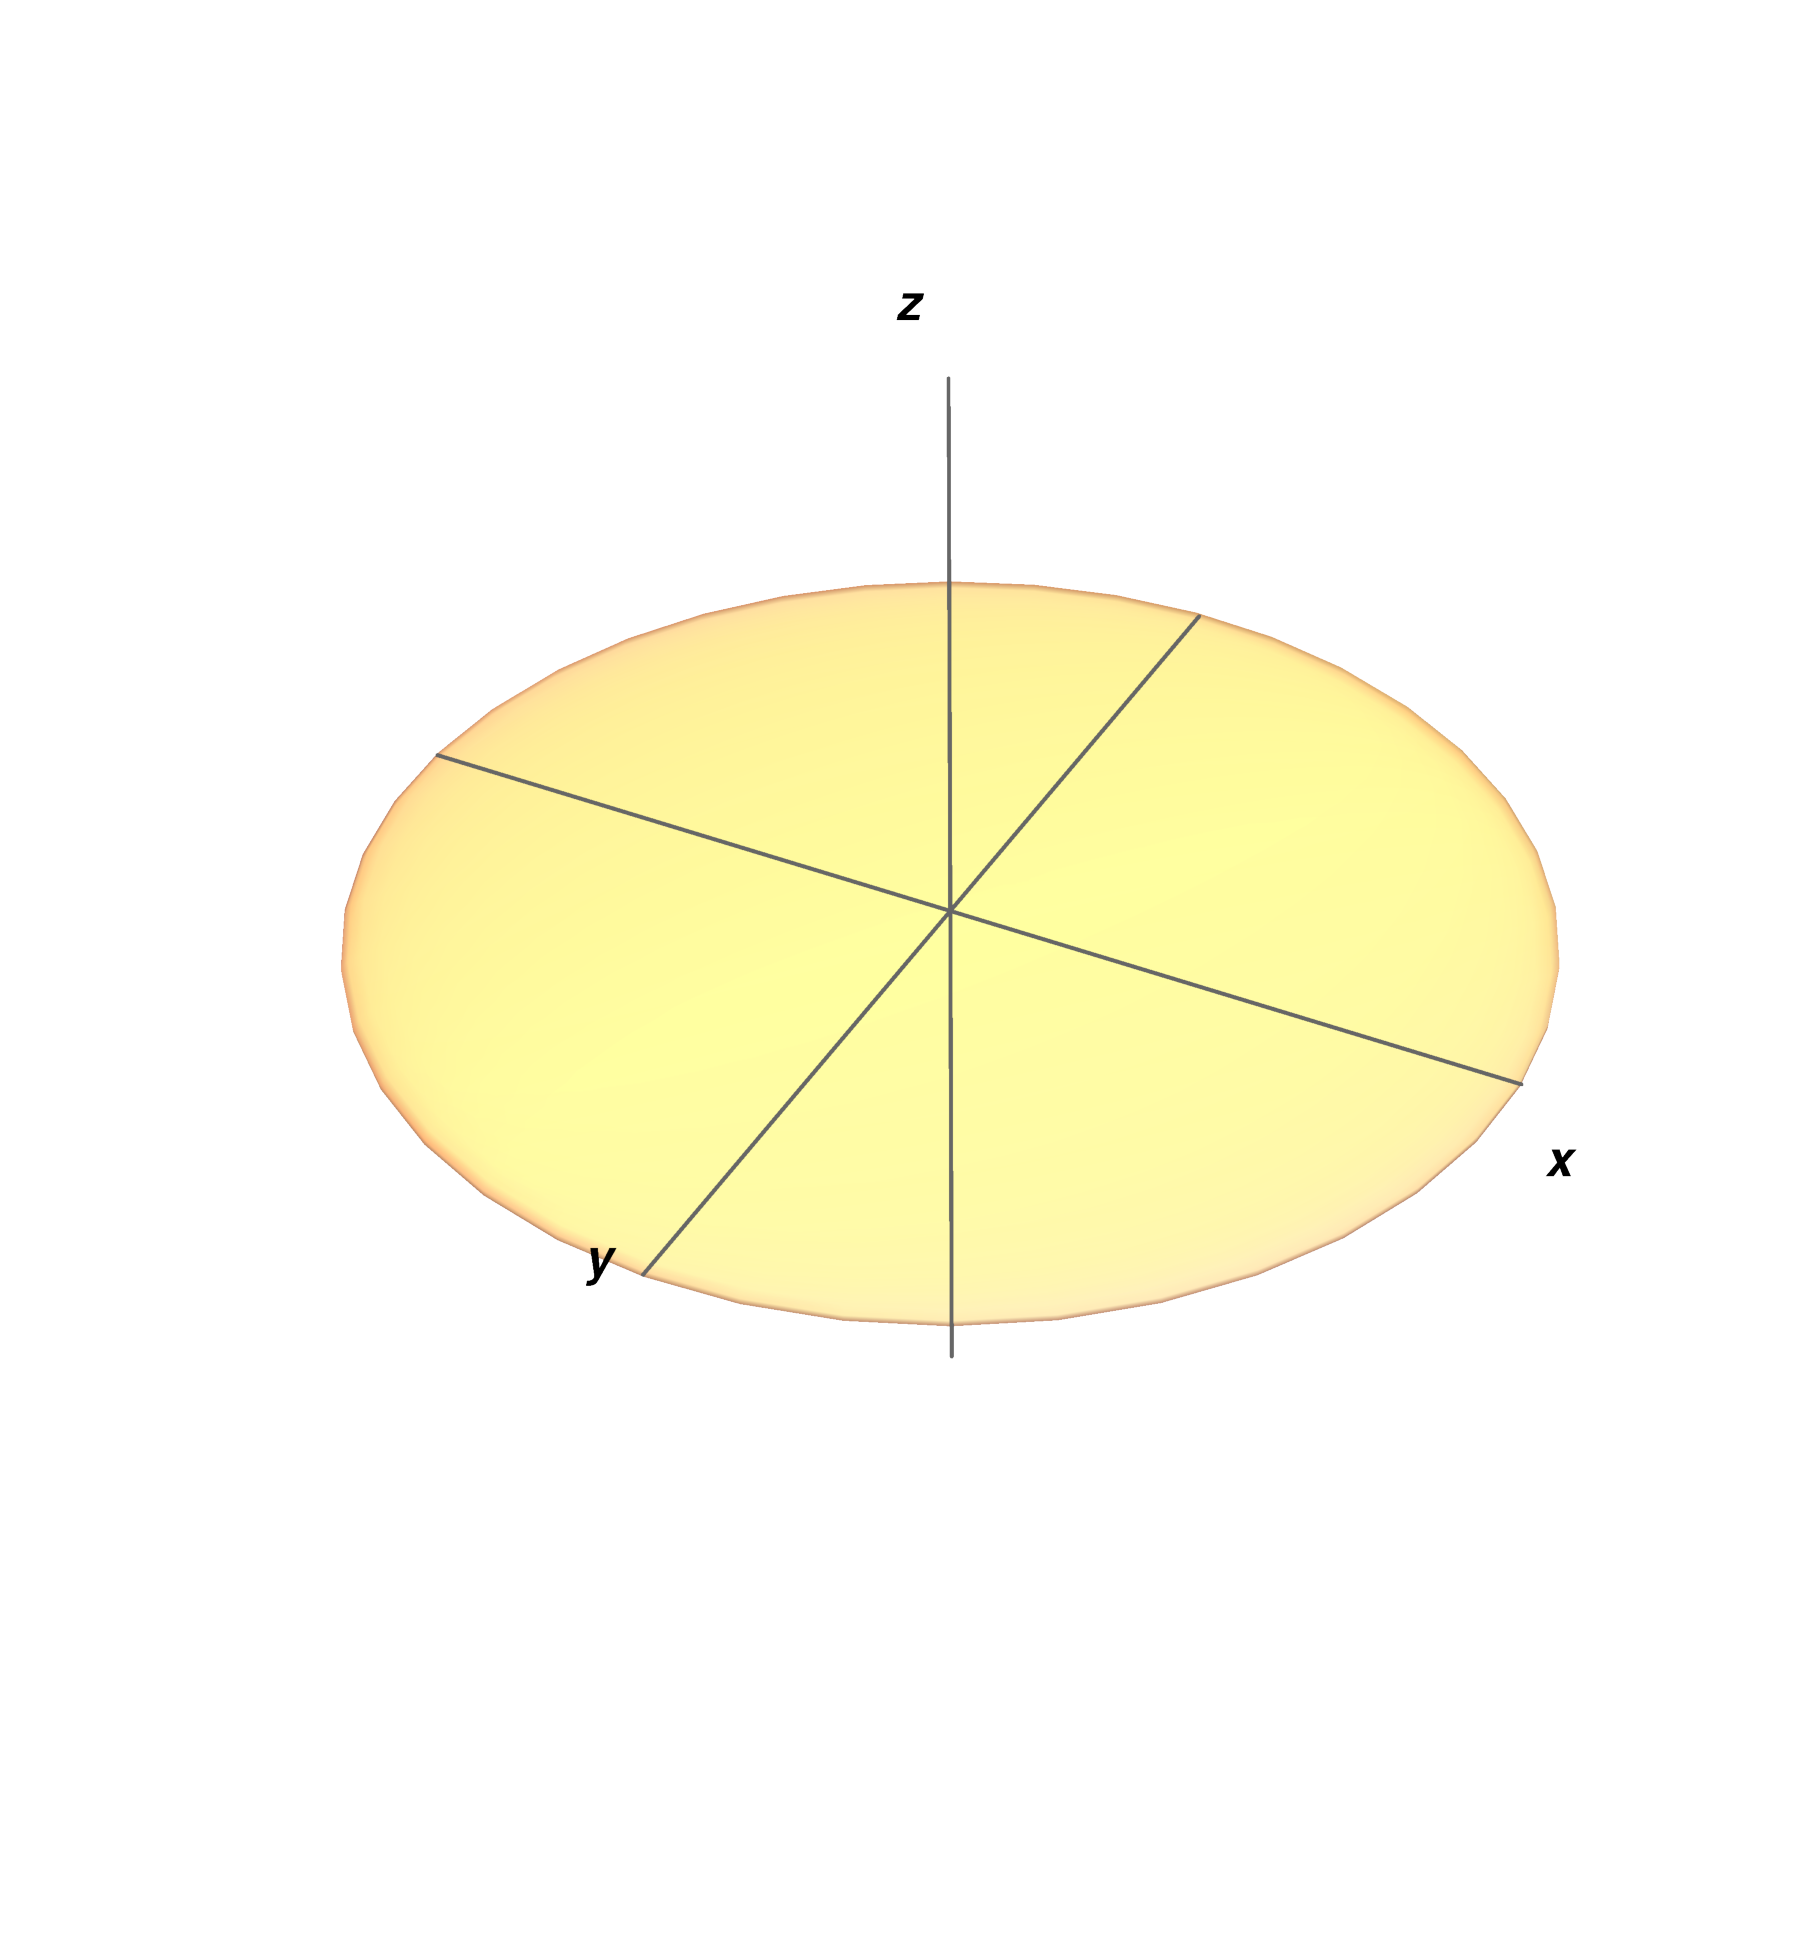
\includegraphics[width=3.5cm]{unit_disk_xy}
	\end{tabular}
	\end{center}
	\vspace{-1cm}
	\begin{align*}
	\qty(1,r_1,r_2,r_3)\longmapsto\qty(1,r_1,r_2,0).
	\end{align*}
	
	\only<1>{	
	$\qty(\Lambda\otimes \mathds{1})\qty[\dyad{\text{Bell}}{\text{Bell}}]\ngeq0$, 
	por consiguiente	$\Lambda$ no es completamente positiva. 
	}
	
	\only<2>{
	\alert{$\qty(\Lambda\otimes \mathds{1})\qty[\dyad{\text{Bell}}{\text{Bell}}]\ngeq0$, 
	por consiguiente	$\Lambda$ no es completamente positiva.}
	}
		
	\vspace{.5cm}
\end{frame}


\begin{frame}{Operaciones PCE}
	Una operación PCE (\textit{Pauli component erasing}) 
	es una operación lineal que transforma a las 	componentes 
	de Pauli de una matriz de densidad $\rho$ de $n$ qubits como
	\begin{align*}
	r_{j_1,\ldots,j_n}\longmapsto \tau_{j_1,\ldots,j_n}r_{j_1,\ldots,j_n},
	\hspace{.8cm}\tau_{j_1,\ldots,j_n}=0,1.
	\end{align*}
	\only<1>{Una operación PCE borra o deja invariantes las componentes de Pauli.}\only<2>{\alert{Una operación PCE borra o deja invariantes las componentes de Pauli. }}\only<3>{Una operación PCE borra o deja invariantes las componentes de Pauli.} 
	
	\hfill
	
\includegraphics[height=2cm]{1qubit_pce_01}
	\hspace{1.8cm}
	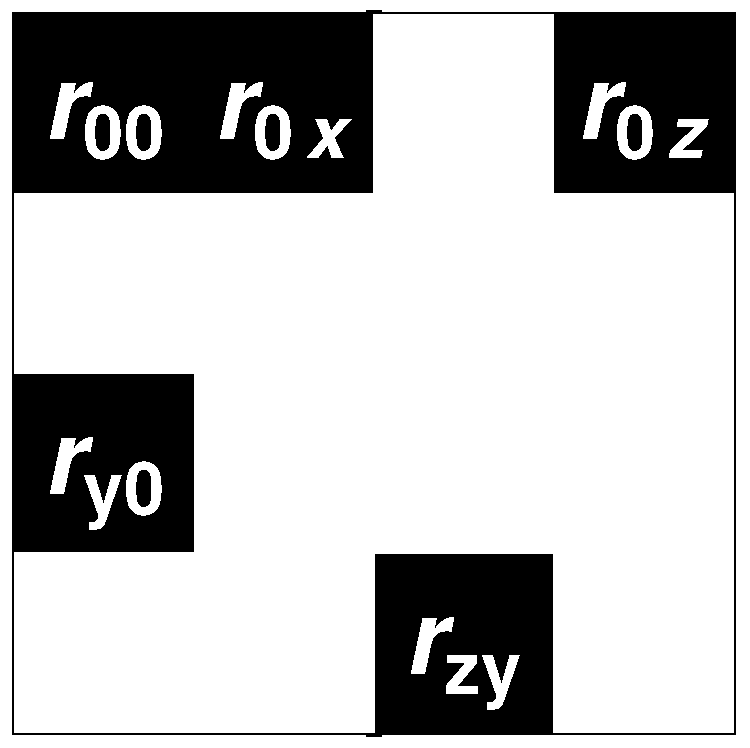
\includegraphics[height=2cm]{2qubit_pce_01}
	\hfill
	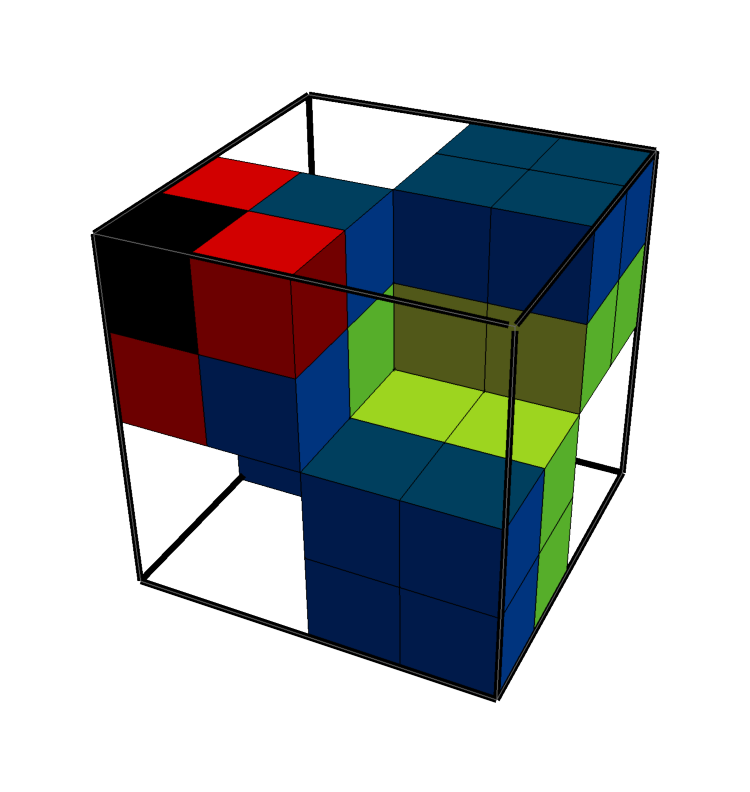
\includegraphics[height=2.5cm]{3qubit_pce_01}
	\hspace{1cm} 

	\vfill	
	
	\only<2>{\textbf{Problema:} ¿cuáles son las características del suconjunto 
	de canales cuánticos de las operaciones PCE?}\only<3>{\alert{	\textbf{Problema:} ¿cuáles son las características del suconjunto 
	de canales cuánticos de las operaciones PCE?}
	}
\end{frame}


\begin{frame}{Canales cuánticos PCE}{Eigenvalores matriz de Choi} 
Los eigenvalores de la matriz de Choi de una operación PCE 
de $n$ qubits son
\begin{align*}
%\qty(\bigotimes_{}^na) \vec{\tau} \geq \vec{0},\\
\vec{\lambda} = 
\underbrace{\qty(a\otimes \ldots\otimes a)}_{n\text{ veces}} \vec{\tau}
\end{align*}
con
\begin{align*}
a=\mqty(1&1&1&1\\1&1&-1&-1\\1&-1&1&-1\\1&1&-1&-1)
\end{align*}
y $\vec{\tau}$ un vector de $4^n$ componentes.
\end{frame}


\begin{frame}{Canales cuánticos PCE}
{Regla $2^k$}
Los canales cuánticos PCE son operaciones que dejan $2^k$ 
componentes de Pauli $r_{j_1,\ldots,j_n}$ invariantes. Sin embargo, 
no sólo importa cuántas $r_{j_1,\ldots,j_n}$, sino también cuáles. 

\vspace{.6cm}

\small{\textbf{\underline{2 qubits, 8 componentes invariantes:}}}

\vspace{.2cm}

\small{
\begin{columns}
\begin{column}{0.5\textwidth}
\hspace{.3cm}
Operaciones PCE que no son\newline
\hspace{.3cm}
canales cuánticos:
\vspace{.1cm}
\begin{center}
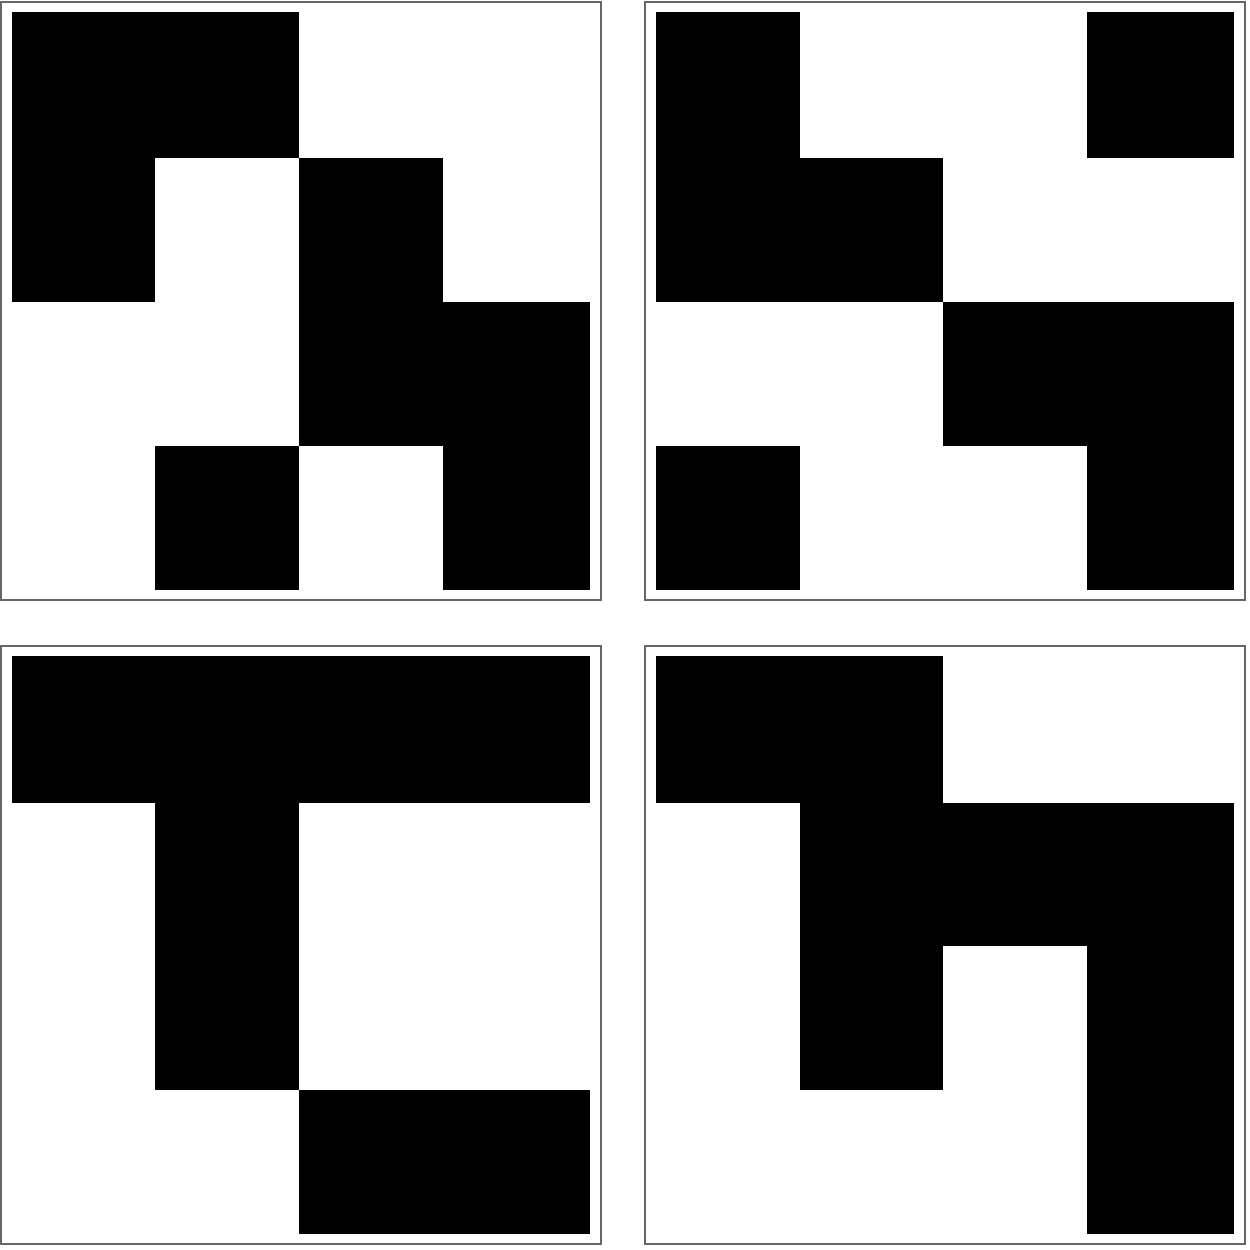
\includegraphics[height=1.8cm]{2qubit_pceOp_8components}
\end{center}
\vspace{1.6cm}
\end{column} 
\begin{column}{0.5\textwidth}
Todos los canales cuánticos PCE que borran 15 componentes:
\begin{center}
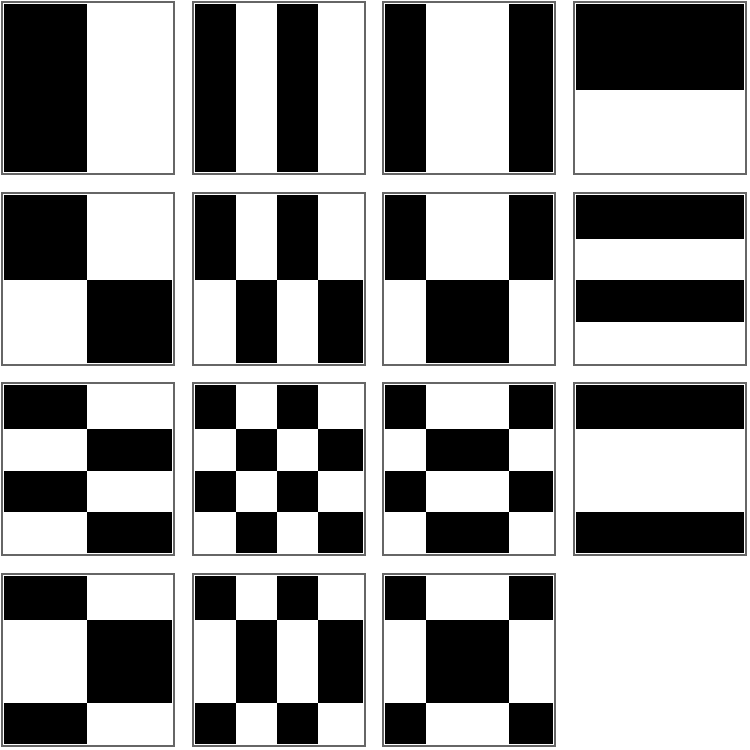
\includegraphics[height=3.8cm]{2qubit_pceQCh_8components}
\end{center}
\end{column}
\end{columns}}
\vspace{2cm}
\end{frame}



\begin{frame}{Canales cuánticos PCE}{Regla espejo}
El número de canales PCE según la cantidad de componentes 
de Pauli invariantes obedece una regla `espejo'.

\vfill

\only<1>{\small{\textbf{\underline{3 qubits:}}}}
\begin{table}[]
\centering
%\begin{tabular}{c|lllll}
%\multirow{3}{*}{\textbf{canales PCE}} &                                &                                & \multicolumn{1}{c}{35}         &                                &                                 \\
%                                                      &                                & \multicolumn{1}{c}{15}         &                                & \multicolumn{1}{c}{15}         &                                 \\
%                                                      & \multicolumn{1}{c}{1}          &                                &                                &                                & \multicolumn{1}{c}{1}           \\
%\hline 
%\textbf{componentes}                                  & \multicolumn{1}{c}{\textbf{1}} & \multicolumn{1}{c}{\textbf{2}} & \multicolumn{1}{c}{\textbf{4}} & \multicolumn{1}{c}{\textbf{8}} & \multicolumn{1}{c}{\textbf{16}}
%\end{tabular}
%\end{table}
%
%\begin{table}[]
%\begin{tabular}{c|lllll}
%\multirow{3}{*}{\textbf{operaciones PCE}} &                                &                                & \multicolumn{1}{c}{455}        &                                &                                 \\
%                                                      &                                & \multicolumn{1}{c}{15}         &                                & \multicolumn{1}{c}{6435}       &                                 \\
%                                                      & \multicolumn{1}{c}{1}          &                                &                                &                                & \multicolumn{1}{c}{1}           \\
%\hline
%\textbf{componentes}                                  & \multicolumn{1}{c}{\textbf{1}} & \multicolumn{1}{c}{\textbf{2}} & \multicolumn{1}{c}{\textbf{4}} & \multicolumn{1}{c}{\textbf{8}} & \multicolumn{1}{c}{\textbf{16}}
%\end{tabular}
\begin{table}[]
\footnotesize
\begin{tabular}{cccccccc}
\multirow{4}{*}{\textbf{canales PCE}} &            &            &            & 1395       &             &             &             \\
                                                      &            &            & 651        &            & 651         &             &             \\
                                                      &            & 63         &            &            &             & 63          &             \\
                                                      & 1          &            &            &            &             &             & 1           \\
\textbf{componentes}                                  & \textbf{1} & \textbf{2} & \textbf{4} & \textbf{8} & \textbf{16} & \textbf{32} & \textbf{64}
\end{tabular}
\end{table}
\end{table} 

\begin{table}[]
\footnotesize
\begin{tabular}{cccccccc}
\multirow{4}{*}{\textbf{operaciones PCE}} &            &            &            & $5.5\times 10^7$ &                     &                         &             \\
                                          &            &            & 39711      &             & $1.2\times 10^{14}$ &                         &             \\
                                          &            & 63         &            &             &                     & $9.2\times 10^{17}$ &             \\
                                          & 1          &            &            &             &                     &                         & 1           \\
\textbf{componentes}                      & \textbf{1} & \textbf{2} & \textbf{4} & \textbf{8}  & \textbf{16}         & \textbf{32}             & \textbf{64}
\end{tabular}
\end{table}

\end{frame}



\begin{frame}{Canales cuánticos PCE}{Generadores}
Los canales cuánticos PCE pueden escribirse como concatenación 
de canales generadores.

\vfill
\small{\textbf{\underline{Generadores canales PCE de 2 qubits:}}}

\begin{center}
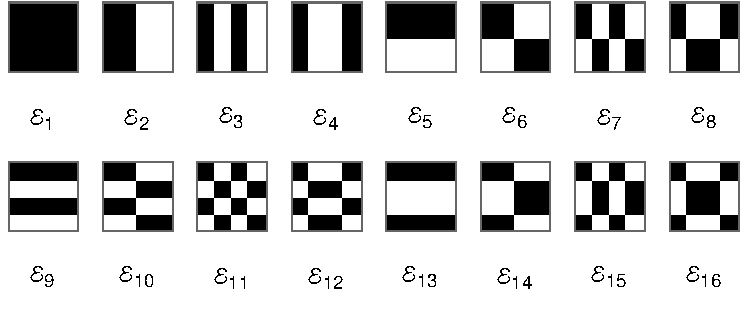
\includegraphics[height=4cm]{2qubits_pce_generators}
\end{center}

\end{frame}




\begin{frame}{Ejemplo}{2 qubits}
\onslide<1->{
\underline{Generadores:}
\begin{center}
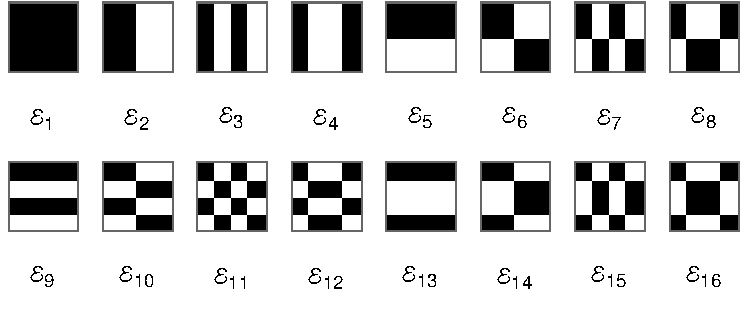
\includegraphics[width=8cm]{2qubits_pce_generators}
\end{center}
}

\onslide<2->{
\hfill
\begin{tabular}{m{0.8cm} m{.1cm} m{0.8cm} m{.05cm} m{0.8cm}}

\includegraphics[height=1.1cm]{E2}  
& $\bigcirc$ 
& 
\includegraphics[height=1.1cm]{E5} 
& $=$
& 
\includegraphics[height=1.1cm]{E2E5} 
\end{tabular} \hspace{1.3cm}
}

\onslide<3->{
\hfill
\begin{tabular}{m{0.8cm} m{.1cm} m{0.8cm} m{.1cm} m{0.8cm} m{.1cm} m{0.8cm}}

\includegraphics[height=1.1cm]{E4}
& $\bigcirc$ 
& 
\includegraphics[height=1.1cm]{E2}  
& $\bigcirc$ 
& 
\includegraphics[height=1.1cm]{E5} 
& $=$
& 
\includegraphics[height=1.1cm]{E4E2E5} 
\end{tabular} \hspace{1.3cm}
}

\onslide<4->{
\hfill
\begin{tabular}{m{0.8cm} m{.1cm} m{0.8cm} m{.1cm} m{0.8cm} m{.1cm} m{0.8cm} m{.1cm} m{0.8cm}}
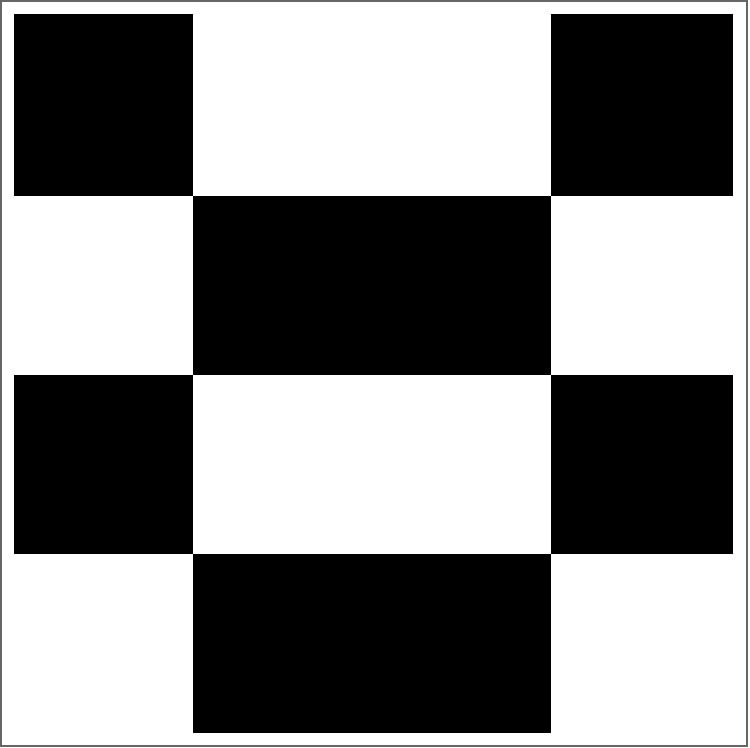
\includegraphics[height=1.1cm]{E12}
& $\bigcirc$ 
& 
\includegraphics[height=1.1cm]{E4}
& $\bigcirc$ 
& 
\includegraphics[height=1.1cm]{E2}  
& $\bigcirc$ 
& 
\includegraphics[height=1.1cm]{E5} 
& $=$
& 
\includegraphics[height=1.1cm]{E12E4E2E5} 
\end{tabular} \hspace{1.3cm}
}
\end{frame}

\begin{frame}{Canales PCE}{$n$ qubits}
%Sea $PCE_n$ al conjunto de canales cuánticos PCE de $n$
%qubits. Existe un conjunto $\Gamma_n\subset PCE_n$ cuyos
%elementos son necesarios y suficientes para generar al resto
%de los elementos en $PCE_n$. \vfill 

%Sea $\mathcal{E}_j\in \Gamma_n$ y $\Phi \in PCE_n$. 
Un canal PCE de $n$ qubits puede escribirse como
\begin{align*}
\Phi = \underbrace{\mathcal{E}_{j_1}\circ \mathcal{E}_{j_2}\circ \ldots
\circ \mathcal{E}_{j_l}}_{\text{máximo }2^n},
\end{align*}
con $\mathcal{E}_{j_i}$ los generadores.

\vfill

\only<1>{
Los generadores $\mathcal{E}_{j_i}$ son las únicas formas que están 
físicamente permitidas de borrar la mitad de las componentes de Pauli 
de un sistema de $n$ qubits.
}
\only<2>{
\alert{
Los generadores $\mathcal{E}_{j_i}$ son las únicas formas que están 
físicamente permitidas de borrar la mitad de las componentes de Pauli 
de un sistema de $n$ qubits.}
}
\end{frame}

% % % % % % % % % % % % % % % % % % % % % % % % % % % % % % % % % % % % % %
% Let's have good manners
% % % % % % % % % % % % % % % % % % % % % % % % % % % % % % % % % % % % % %
\begin{frame}
  \begin{center}
    ¡Muchas gracias!

    \vfill

    Contacto:

    José Alfredo de León

    deleongarrido.jose@gmail.com
  \end{center}
\end{frame}

\end{document}

%%% Local Variables:
%%% mode: latex
%%% TeX-master: t
%%% End:
